\documentclass[tikz]{standalone}
\usepackage{pgfplots}
\pgfplotsset{compat=1.15}
\usepackage{mathrsfs}
\usetikzlibrary{arrows,calc}
\usepackage{tkz-euclide}
\pagestyle{empty}

\definecolor{AngleClr}{rgb}{0,0.39215686274509803,0}
\definecolor{ShapeClr}{rgb}{0.6,0.2,0}
\definecolor{BlueClr}{RGB}{13,93,184}

\begin{document}

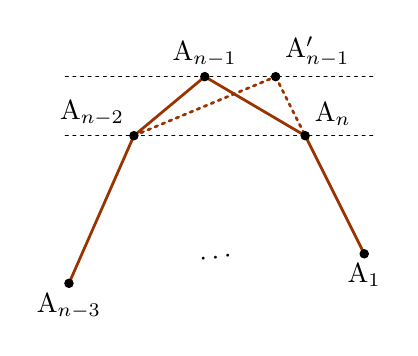
\begin{tikzpicture}[scale=.75]
\tkzSetUpLine[line width=1pt,color=black]
\tkzSetUpPoint[fill=black]

\tkzDefPoints{-0.5/0/a3,0.6/2.5/a2,1.8/3.5/a1,3.5/2.5/a0,4.5/0.5/A1,0.6/3.5/b2,3.5/3.5/b0}

\tkzFillPolygon[fill=white,fill opacity=0.2](a3,a2,a1,a0,A1)

\tkzDrawSegments[line width=1pt,color=ShapeClr](a3,a2 a2,a1 a1,a0 a0,A1)
\tkzDrawSegments[line width=0.5pt,color=black,dashed,dash pattern=on 1pt off 1.75pt,add=0.4 and 0.4](a2,a0 b2,b0)

\tkzInterLL(b0,b2)(a0,A1) \tkzGetPoint{b1}
\tkzDrawSegments[line width=1pt,color=ShapeClr,dashed,dash pattern=on 1pt off 1.75pt](a2,b1 b1,a0)

\tkzDrawPoints[size=3](a3,a2,a1,a0,A1,b1)


\tkzLabelPoint[below](a3){${\rm A}_{n-3}$}
\tkzLabelPoint[above left](a2){${\rm A}_{n-2}$}
\tkzLabelPoint[above](a1){${\rm A}_{n-1}$}
\tkzLabelPoint[above right](a0){${\rm A}_{n}$}
\tkzLabelPoint[below](A1){${\rm A}_1$}
\tkzLabelPoint[above right](b1){${\rm A}_{n-1}'$}

\tkzLabelSegment[above,sloped,pos=0.5](a3,A1){$\ldots$}

\end{tikzpicture}

\end{document}
